\chapter{Experiment}
In this chapter, I describe the details about the experiment to find correlations between the data gathered from the mobile devices and the code quality. It shows the execution of the experiment as well as the usage of the gathered data and interpretation. 

\section{Crowd Experiment}

\begin{figure}
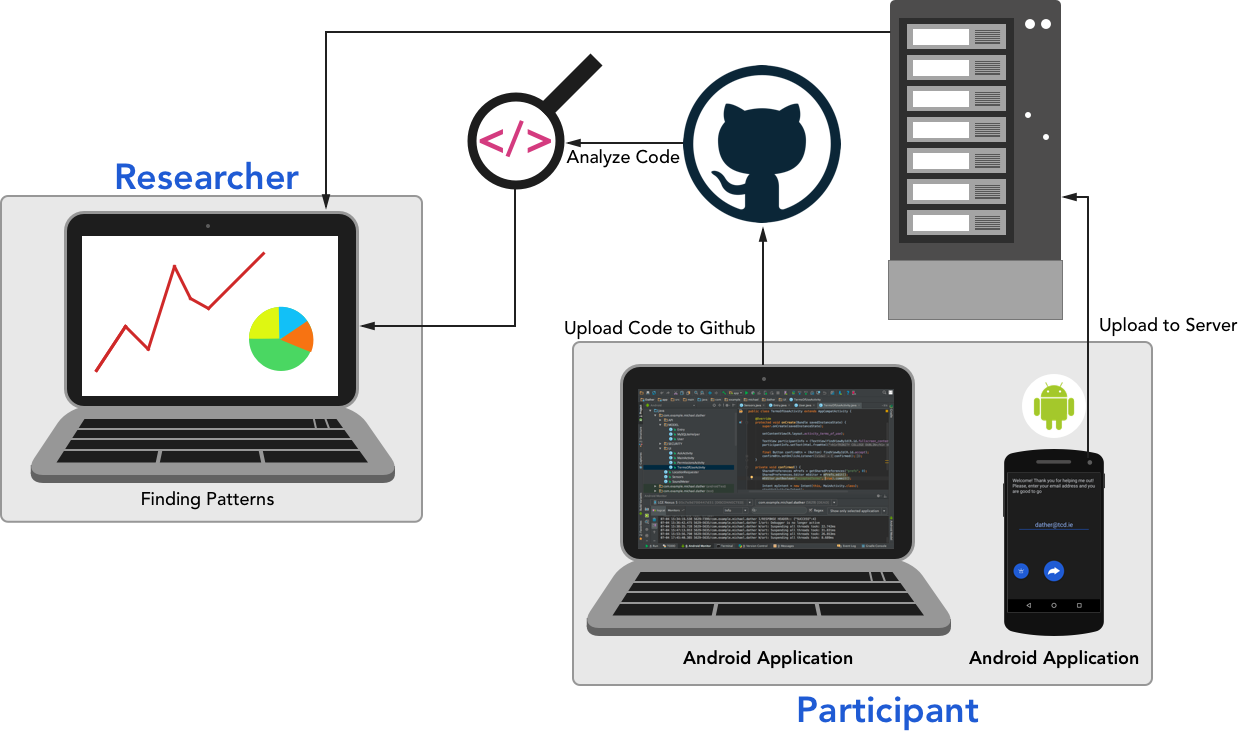
\includegraphics[width=\textwidth]{experiment}
\caption{Experiment Execution}\label{experiment}
\vspace{10 mm}
\end{figure}

In the experiment, participants are solving a programming task while the Dather Android App is running to record behavior and environmental factors. After the submitted code is been analyzed, it has been compared with the gathered data in order to find correlations between the participants performance and the information from the gathered data. You can see the flow of the experiment in Figure \ref{result}. 
\subsection{Setup and Execution}
Every participant needs to have access to a mobile phone with Android version 4.4 or later. In order to take part at the experiment, a participant needs to install the Dather Application of his/her device. The Application can be downloaded from the website \url{http://frickm.de} when it's been accessed from the Android device. 
\bigbreak
After installing the downloaded apk-file, the participant gives permissions within the application to gather the data and allows the data to be used for research. 
As the last step before being able to start the experiment, the user needs to enter his/her email address.\\
After setting up the application and accessing the website which contains the programming task, the experiment is ready to start. The participant runs the gathering process while working on the programming task.\\
After completing the task, the participant uploads the solution code to Github and sends a link of the Github repository from the Email address. The github account name can later be used to match the gathered data with the uploaded solution-code of the participant. 

\subsection{Classification}
With the result values it might there might occur correlations between the entries and the coding quality. However, that approach is not using the full capability. In order to understand the values rather than just using them, it makes sense to interpret them and bring it into a context. Previous research results and also classifying controlled tested events using the gathered values will be described in further detail within the next paragraphs.

\subsubsection{Indoor Outdoor differentiation}
The brightness of indoor lightning is different from the brightness outdoors. Indoor environments are mostly receiving light from an artificial light source which flickers in a rate than can't be noticed by the human eye. Sadly the light sensor of the mobile devices is not precise enough to detect that flickering. Anyhow, also the luminance is different indoors and outdoors. Artificial lights are just not as powerful as the sun and it would require a ridiculous amount of artificial light sources and windows to create the same brightness within buildings as they are outside. 
As seen in the two tables \ref{outLight} and \ref{inLight} based on the lux from the light sensor it is possible to detect whether the device is indoor or outdoor by a high probability.

%%%% TABLE outdoor light
\setlength{\tabcolsep}{10pt}
\renewcommand{\arraystretch}{1.5}
{\rowcolors{3}{black!10!white!90}{white!100}

\begin{table}[!htb]
\centering
\begin{tabular}{ |p{4cm}|p{4cm}|  }
 \hline
 \rowcolor{lightgray} \multicolumn{2}{|c|}{{\bf Common Light Levels Outdoor - Daytime}} \\
 \hline
{\bf Condition} & {\bf Illumination in lux}\\
 \hline
 Sunlight   		& 107,527\\
 Full Daylight   	& 10,752.7\\
 Overcast Day	& 1,075.3\\
 Very Dark Day	& 107,527\\
 \hline
\end{tabular}
\caption{Common Outdoor Light Levels}
\label{outLight}
\end{table}

%%%% TABLE indoor light
\begin{table}[!htb]
\centering
\begin{tabular}{ |p{10cm}|p{4cm}|  }
 \hline
 \rowcolor{lightgray} \multicolumn{2}{|c|}{{\bf Common and Recommended Light Levels Indoor}} \\
 \hline
{\bf Activity/Location} & {\bf Illumination in lux}\\
 \hline
 Warehouses, Homes, Theaters, Archives   																	& 150\\
 Easy Office Work, Classes   																						& 250\\
 Normal Office Work, PC Work, Study Library, Groceries, Show Rooms, Laboratories	& 500\\
 Supermarkets, Mechanical Workshops, Office Landscapes 											& 750\\
 Normal Drawing Work, Detailed Mechanical Workshops, Operation Theatres 				& 1,000\\
 Detailed Drawing Work, Very Detailed Mechanical Works 											& 1,500 - 2,000\\
 \hline
\end{tabular}
\caption{Common \& Recommended Indoor Light Levels}
\label{inLight}
\end{table}

\FloatBarrier
\clearpage

\subsubsection{Usage of Mobile Phone}
The Y and Z axis of the 3D accelerometer can be used to detect whether the participant uses his phone. The simple classification picks up the change between the mobile device laying flat on the desk and the device being in a vertical position which is the position it would be when the user holds it in his/her hand. The graphic \ref{accDev} shows shows the two states and the changes in the Y and Z-axis values. 

\begin{figure}[!htb]
\centering
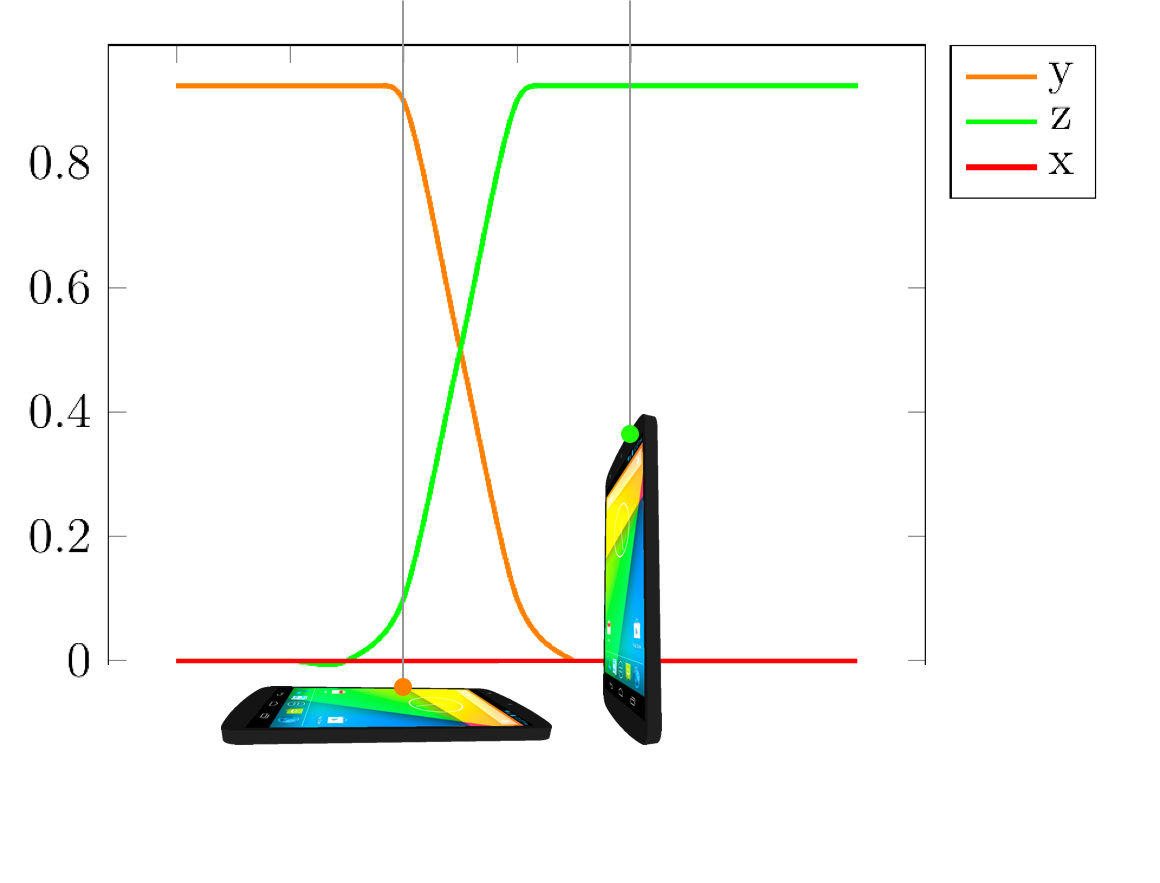
\includegraphics[width=10cm]{accDevice}
\caption{Android Views}\label{accDev}
\vspace{10 mm}
\end{figure}

\FloatBarrier

\subsubsection{Guessing the users location}
In order to guess the location of the user, the location with the environmental noise as well as the detection whether the user is indoor our outside. The location accuracy depends on the way how it is been calculated which is ether the network or GPS. However, it can vary and can't ensure a perfect detected location but using the noise and indoor/outdoor information can help to limit the results to less possibilities. When, for example the location shows a radius in an area with a library, a coffee shop and a public crowded square it's a high chance that the library is not an option in the case of a noisy environment. In order to detect whether the user is in the coffee-shop or the square, the light sensor can detect whether the light value is in the outdoor or indoor brightness range. 

\subsubsection{Movement}
The movement of the user can directly be seen by the steps he/she walks during the start of the gathering until the ending. The distance and the frequency shows if the user just walks to the fridge, toilet or somewhere close or actually walks from one place to another. Also the locations can indicate that. 
The location can also show whether the user was on public transport, on a train/car or an Airplane depending on the travel speed and from where the user started and where he/she arrives (airport, garage, train-station etc.). 

\subsubsection{Weather Conditions}
With the location and the timestamps of the gathering and it is possible to get information about the local weather of the users location at the time when the gathering happend using the website   http://www.timeanddate.com/weather \cite{weatherArchive}.

\subsubsection{Music}
Using the environmental noise it is possible to find patterns that can be related to music. In general modern music has a very constant noise level rather than the dynamic classical music. The iTunes top 100 songs at July 14th 2016 have an average length of 3:39 minutes, the shortest song is 2:42 minutes and the longest 5:13 minutes long.
In order to detect whether the participant is listening to music the volume should go down for 2-5 seconds between a track with a duration between 2:30 minutes and 5:30 minutes. 
A regular pattern with these attributes should indicate that the user is listening to background music while working on the coding task.

\subsection{Questions}
After the gathering process, the participant is asked to answer some questions:
\begin{itemize}
\item Are you a Student?
\item Did you work in a team?
\item Did you listen to music?
\item Did you feel tired?
\item Did you enjoy the tasks?
\item Did you give all you attention to the tasks?
\item Were you distracted during the tasks?
\item Did you feel stressed
\item Do you think the tasks were easy?
\end{itemize}

All the questions can either be checked to indicate 'yes' or leave unchecked for 'no'. The answers can help to clarify the classification or to get new additional contexts. Some of the questions are created based on the knowledge from previous work of researchers and their results that can possibly influence cognitive performance. 
In a long term, asking questions is not optimal. In the future the app is supposed to learn and slowly make the questions unnecessary. Currently there is a way to detect whether the user is listening to music by identifying patterns but the accuracy is not exactly known and therefore also asked as a question as well could it be that the user is wearing headphones. If the detection using the environmental noise is highly accurate, the question can be removed from the app.
 
 
\section{Individual Experiment}
The purpose of the second experiment is to find evidence of specific factors that influence the ability of cognitive thinking. Different isolated scenarios are been tested by a participant in order to find correlations between the specific environments. 
This experiment allows to test the factors in a more controllable environment but based on one individual person. 

\subsection{Setup and Execution}
In this experiment a participant solved some cognitive tasks while being in a controlled environment in order to test the performance influences of isolated factors. 
Of course it is very unlikely or even impossible to test a factor in complete isolation one factor. There are always side factors that which are unavoidable. They could be for example the human itself, sudden unpredictable changes in the environment and of course the problem in keeping the factors of one part of the measurement equal to the factors of other measurements. 
To minimize these factors, the 'Dather' Android application helped to monitor the environment and remove recorded tasks where the environment information are too different of results which are were correlated with each other. 
However, with this problems in mind, the idea to measure changes in the cognitive performance of a person, was measuring the time of finishing a Sudoku game. 
The game, where the goal is to systematically add missing numbers in a 9x9 matrix, requires concentration and logical combining of numbers. 
The sudoku game was already used in previous research for measuring the cognitive performance \cite{sobolewski2009monitoring} \cite{xiang2009using}. 
Another reason for using Sudokus is that they can be randomly generated with a specific calculated difficulty level to make sure that every Sudoku is equally hard to solve. 
A website \cite{sudokugen} generated the Sudokus uses an engine which is part of the gnome-sudoku software \cite{gnomeSudoku}. 
A medium difficulty level and a limited calculated range of difficulty to +/- 0.02 of 0.5 was the base for generating the Sudokus which were then printed on paper, one per page. 

\subsection{Scenarios}
The following scenarios have been tested. Each scenario was performed 10 times to get a good mean which decreases the randomness in the experiment. In order to control the environment variables, a modified version of the Android app recorded the environmental light and volume and it was made sure that the values don't differ much to have a influence in the results. 
The experiments were executed over a several days in mixed up order to avoid that the training-process in solving the Sudokus can also influence the overall average of the outcomes.

\subsubsection{Music}
The scenarios to compare in this part the influence of two different types of music and as a control scenario no music at all. The participant did the Sudokus while listening to Spotify-Radio \cite{spotify} 'Heavy Metal' and 'Classical' over headphones on a defined level of volume. In the control case without music, the participant was not wearing headphone but working in a very quite environment.

\subsubsection{Coffee}
In this scenario I wanted to test the influences of Coffee in the cognitive performance as discovered by Watters, Paul Andrew et. al. \cite{watters1997caffeine}. Simultaneously to their results I used a caffeine level of almost the value that they found out is the optimum for cognitive performance (400 mg). 
The whole experiment was executed in 5 days in a row with two tasks before, and two tasks after having a coffee. 
First, the participant solved the Sudokus without taking any caffeine for more than 16 hours, which is more than enough to make sure no other caffeine intake can influence to experiment \cite{liguori1997absorption}. Additionally the participant had the same breakfast every day before every experiment. 
For the second part of the experiment, the participant had the coffee drink that contained hot water with 5 espresso shots from Starbucks. The Coffee Franchise declares one espresso with 75mg caffeine each, which sums our drink up to 375mg at an amount of 5. After having the coffee, the participant waited 40 minutes for the caffeine to be absorbed \cite{liguori1997absorption} and started with the Sudoku. 

